% !TEX TS-program = pdflatex
% !TEX root = tesi.tex

\documentclass[
  a4paper,
  twoside,
  openright,
  titlepage,
  headinclude,
  footinclude,
  BCOR5mm,
  numbers=noenddot,
  cleardoublepage=empty,
  tablecaptionabove
]{scrreprt}

\usepackage[T1]{fontenc}
\usepackage[utf8]{inputenc}
\usepackage{amsmath,amssymb}
\usepackage{indentfirst}
\usepackage[
  style=philosophy-modern,
  hyperref
]{biblatex}
\usepackage{chngpage}
\usepackage{calc}
\usepackage{listings}
\usepackage{graphicx}
\usepackage{subfig}
\usepackage{lipsum}
\usepackage{shapepar}
\usepackage{pifont}
\usepackage[
  eulerchapternumbers,
  subfig,
  beramono,
  eulermath,
  pdfspacing,
  listings
]{classicthesis}
\usepackage{arsclassica}

% FONT UTILIZZATO DAL CONSERVATORIO
\usepackage[defaultfam,tabular,lining]{montserrat} %% Option 'defaultfam'
%% only if the base font of the document is to be sans serif
\usepackage[T1]{fontenc}
\renewcommand*\oldstylenums[1]{{\fontfamily{Montserrat-TOsF}\selectfont #1}}

\usepackage{ccicons}

% ********************************************************************
% Personal commands
% ********************************************************************
\DeclareRobustCommand*{\clsname}[1]{{\normalfont\sffamily#1}}
\DeclareRobustCommand*{\pkgname}[1]{{\normalfont\sffamily#1}}
\DeclareRobustCommand*{\optname}[1]{{\normalfont\ttfamily#1}}
\DeclareRobustCommand*{\cmdname}[1]{\mbox{\lstinline[basicstyle=\normalsize\ttfamily]!\\#1!}}

\DeclareRobustCommand*{\classicthesis}{Classic\-Thesis}
\DeclareRobustCommand*{\arsclassica}{{\normalfont\sffamily ArsClassica}}

% ********************************************************************
% Hyper-references
% ********************************************************************
\newcommand{\mail}[1]{\href{mailto:#1}{\texttt{#1}}}


% ********************************************************************
% Graphics
% ********************************************************************
\graphicspath{{Graphics/}}


% ********************************************************************
% Code
% ********************************************************************
\definecolor{lightergray}{gray}{0.99}
\definecolor{bbari}{cmyk}{1,0.44,0,0.28}

\lstset{language=[LaTeX]Tex,
     keywordstyle=\color{RoyalBlue},
     basicstyle=\small\ttfamily,
     commentstyle=\color{Emerald}\ttfamily,
     stringstyle=\rmfamily,
     numberstyle=\scriptsize,
     showstringspaces=false,
     breaklines=true,
     frame=lines,
     backgroundcolor=\color{lightergray},
     flexiblecolumns=true,
     escapeinside={�*}{*�},
     firstnumber=last,
}

\newcommand{\meta}[1]{$\langle${\normalfont\itshape#1}$\rangle$}

\lstset{	morekeywords=%
    {ProvidesPackage,RequirePackage,areaset,ifthenelse,%
     chapterNumber,undefined,boolean,DeclareRobustCommand,%
     spacedallcaps,textssc,MakeTextUppercase,lehead,%
     microtypesetup,textls,spacedlowsmallcaps,MakeTextLowercase,%
     sodef,allcapsspacing,lowsmallcapsspacing,thesection,%
     color,headmark,rohead,headfont,pnumfont,titleformat,%
     part,partname,thepart,chapter,thechapter,titlerule,%
     subsection,thesubsection,subsubsection,thesubsubsection,%
     paragraph,theparagraph,descriptionlabel,titlespacing,%
     formatchapter,textcolor,clearscrplain,rofoot,labelitemi,
     captionsetup,hypersetup}}

\lstnewenvironment{code}%
   {\setkeys{lst}{columns=fullflexible,keepspaces=true}%
   \lstset{basicstyle=\small\ttfamily}}{}


% ********************************************************************
% Bibliography
% ********************************************************************
\bibliography{Bibliography}

\defbibheading{bibliography}{%
\cleardoublepage
\manualmark
\phantomsection
\addcontentsline{toc}{chapter}{\tocEntry{\bibname}}
\chapter*{\bibname\markboth{\spacedlowsmallcaps{\bibname}}
{\spacedlowsmallcaps{\bibname}}}}

\renewcommand*{\nameyeardelim}{\addcomma\space}


\newcommand{\myName}{Albert Einstein}
\newcommand{\myTitle}{Theory of relativity}
\newcommand{\mySubTitle}{Introduction to general relativity}

\begin{document}
\pagenumbering{roman}
\pagestyle{plain}
% !TEX TS-program = pdflatex
% !TEX root = ../tesi.tex

%*******************************************************
% Titlepage
%*******************************************************
\begin{titlepage}
\pdfbookmark{Titlepage}{Titlepage}
\changetext{}{}{}{((\paperwidth  - \textwidth) / 2) - \oddsidemargin - \hoffset - 1in}{}
  \begin{center}
    {\LARGE
      
\includegraphics[width=0.641\textwidth]{logo.eps} \\[0.5cm]

      {\normalsize{DIPARTIMENTO DI NUOVE TECNOLOGIE E LINGUAGGI MUSICALI}} \\[-0.2cm]
      {\spacedlowsmallcaps{Scuola di Musica elettronica}} \\[0.5cm]

      {\normalsize{DIPLOMA ACCADEMICO DI PRIMO LIVELLO IN}} \\[-0.2cm]
      %{\spacedlowsmallcaps{Tecnico del Suono}} \\[1.414cm]
      {\spacedlowsmallcaps{Musica Elettronica}} \\[1.414cm]

      {\huge{\spacedlowsmallcaps{\myName}}}\vspace{-0.3cm}
      \par\noindent\rule{\textwidth}{0.4pt}\vspace{0.3cm}
      {\Huge{\color{bbari}\spacedallcaps{\myTitle}}}
      \par\noindent\rule{\textwidth}{0.4pt}\vspace{0.3cm}
      {\spacedlowsmallcaps{\mySubTitle}}
    }

    \vspace{2.718cm}

    \begin{minipage}[t]{0.49\textwidth}
    \begin{flushleft} \large
    \emph{Autore:}\\
    \spacedlowsmallcaps{\myName}\\
    \spacedlowsmallcaps{1234/T}
    \end{flushleft}
    \end{minipage}
    \begin{minipage}[t]{0.49\textwidth}
    \begin{flushright} \large
    \emph{Relatore:} \\
    \spacedlowsmallcaps{Prof. Giuseppe Silvi}\\
    \spacedlowsmallcaps{Elettroacustica}
    \end{flushright}
    \end{minipage}\\[0.5cm]
    \begin{minipage}[t]{0.99\textwidth}
    \begin{flushright} \large
    \emph{Correlatore:} \\
    \spacedlowsmallcaps{Luigi Nono}\\
    \spacedlowsmallcaps{Compositore}
    \end{flushright}
    \end{minipage}\\[3cm]

    \vfill

    ANNO ACCADEMICO 2021/22

  \end{center}
\end{titlepage}

% !TEX TS-program = pdflatex
% !TEX root = ../tesi.tex

%*******************************************************
% Titleback
%*******************************************************
\thispagestyle{empty}
\pdfbookmark{Titleback}{Titleback}

\hfill

\vspace{\stretch{2}}

\begin{center}
\myName \\
\smallskip
\textit{\myTitle}\\
\smallskip
Copyright \ccbyncsa\\
2022-2023
\end{center}
\vspace{\stretch{1}}

\medskip

\noindent\textsf{\spacedlowsmallcaps{Disclaimer}} \\
\noindent
This document was written with \LaTeX{} on Mac using \arsclassica, a reworking of the \classicthesis{} style designed by Andr\'e Miede, inspired to the masterpiece \emph{The Elements of Typographic Style} by Robert Bringhurst.

\bigskip

\noindent This work is licensed under a Creative Commons\\
Attribution-NonCommercial-ShareAlike 4.0 International License.

\bigskip

\noindent
\textsf{\spacedlowsmallcaps{Contacts}}

\noindent
{\raisebox{-0.33ex}{\ding{43}}}\,\mail{albert.einstein@gmail.com}

\cleardoublepage
% !TEX TS-program = pdflatex
% !TEX root = ../tesi.tex

%*******************************************************
% Acknowledgements
%*******************************************************
\pdfbookmark{Acknowledgements}{Acknowledgements}

\chapter*{Acknowledgements}

\begin{flushright}
\itshape
We have seen that computer programming is an art, \\
because it applies accumulated knowledge to the world, \\
because it requires skill and ingenuity, \\
and especially because it produces objects of beauty. \\
\medskip
--- Donald Ervin Knuth
\end{flushright}

\bigskip
\bigskip

\heartpar{I wish first of all to thank the members of the Italian \TeX{} and \LaTeX{} User Group, in particular
Claudio Beccari, Fabiano Busdraghi, Gustavo Cevolani, Rosaria D'Addazio, Agostino De Marco, Massimiliano Dominici, Gloria Faccanoni, Claudio Fiandrino, Heinrich Fleck, Enrico Gregorio, Massimo Guiggiani, Roberto Giacomelli, Gianluca Gorni, Maurizio Himmelmann, Jer\'onimo Leal, Paride Legovini, Lapo Filippo Mori, Gianluca Pignalberi, Luigi Scarso, Marco Stara, Andrea Tonelli, Ivan Valbusa, Emiliano Giovanni Vavassori and Emanuele Vicentini,
for their invaluable aid during the writing of this work, the detailed explanations, the patience and the precision in the suggestions, the supplied solutions, the competence and the kindness: thank you, guys!
Thanks also to all the people who have discussed with me on the forum of the Group, prodigal of precious observations and good advices.
Finally, thanks to Andr\'e Miede, for his wonderful ClassicThesis style, and to Daniel Gottschlag, who gave to me the hint for this original reworking.}

\pagestyle{scrheadings}
% !TEX TS-program = pdflatex
% !TEX root = ../tesi.tex

%*******************************************************
% Contents
%*******************************************************
\phantomsection
\pdfbookmark{\contentsname}{tableofcontents}
\setcounter{tocdepth}{2}
\tableofcontents
\markboth{\spacedlowsmallcaps{\contentsname}}{\spacedlowsmallcaps{\contentsname}}

\cleardoublepage
\pagenumbering{arabic}
% !TEX TS-program = pdflatex
% !TEX root = ../tesi.tex

%************************************************
\chapter{Fundamentals}
\label{chp:fundamentals}
%************************************************

This chapter introduces the (truly simple) basic notions of \arsclassica{} and presents its fundamental ideas and distinctive features.



\section{Introduction}

The \arsclassica{} package changes some features of the \classicthesis{} style, designed by Andr\'e Miede. It allows to reproduce the layout of the \LaTeX{} guide \emph{The Art of Writing with \LaTeX}~\parencite{pantieri:arte} and of this document.

\section{Use}

This package is shaped to be executed on a \emph{complete} installation of \TeX{}~Live or MiK\TeX, and uses freely available fonts.
It works with the \clsname{KOMA-Script} classes (\clsname{scrreprt}, \clsname{scrbook} and \clsname{scrartcl}) and requires the \pkgname{classicthesis} package. \arsclassica{} must be loaded \emph{after} \pkgname{classicthesis}:
\begin{code}
\documentclass[\meta{\dots\unkern}]{scrreprt} % or scrbook or scrartcl

\usepackage[\meta{\dots\unkern}]{classicthesis}
\usepackage{arsclassica}

\begin{document}
\dots
\end{document}
\end{code}

For example, this document has been produced with the following code:
\begin{code}
\documentclass[a4paper,twoside,openright,titlepage,
               headinclude,footinclude,BCOR5mm,
               numbers=noenddot,cleardoublepage=empty,
               tablecaptionabove]{scrreprt}

\usepackage{\meta{\dots\unkern}}
\usepackage{subfig}
\usepackage[eulerchapternumbers,subfig,beramono,eulermath,pdfspacing]%
           {classicthesis}
\usepackage{arsclassica}

\begin{document}
\dots
\end{document}
\end{code}

It is recommended to use the \optname{beramono} and \optname{eulerchapternumbers} options together with \arsclassica.



\section{Style}

The typographical style achieved with \arsclassica{} differs from \classicthesis{} in the following points:
\begin{itemize}
\item use of Iwona font, by Janusz Nowacki, for the sectioning unit titles (chapters, sections, subsections, sub-subsections, paragraphs and subparagraphs), for the description list labels, the headlines and the caption labels (\classicthesis{} doesn't use any sans serif font);
\item customized chapter numbers;
\item semi-transparent headlines; the headlines are separated from the page number by a small rule;
\item caption labels in boldface (\classicthesis{} doesn't use any boldface font);
\item itemize lists with semi-transparent bullets.
\end{itemize}

\arsclassica{} is designed  to provide a ready-to-use typographical style: for this reason it has no loading options and it is \emph{not} configurable or customizable in any way. If you change the previous settings, you'll risk to destroy the balance of the style, so it is \emph{highly recommended} to keep them unchanged.

One of the principles of \LaTeX{} is that it allows the author to take no interest in the typographical questions, permitting him to focus only on the structure and the contents of his document. This fact should always be kept in mind: using a style written by others, the user accepts all the typographical settings chosen for him by the author of the style, and he isn't forced to study typography to fine-tune the layout of his publications. This is the case of \arsclassica{} too: if you change its settings, you'll deny this philosophy and, consequently, you'll have to study (a lot of) typography to achieve acceptable results.

The style achieved with \arsclassica{} is \emph{not} therefore configurable or customizable. The typographical style is very personal: if you like this package and find attractive the idea to take no interest in the problem of the style definition, then you'll use \arsclassica{} with satisfaction; otherwise, if you have different needs or you aren't satisfied with the layout of the package, then you should try other classes or packages, even building your own style.



\section{Important}

To write a document according to the \arsclassica{} style, you have to follow some very simple rules.
\begin{itemize}
\item Don't change \emph{for any reason} the \arsclassica{} settings (fonts, text body size, colors, \dots).
\item The sectioning unit titles (chapters, section, subsections, \dots) have to be \emph{one line long}, possibly in \emph{plain text} (no symbols, formulas or code fragments). If you have titles longer than one line, try and rephrase them: you can almost always do it.
\item In the table of contents and in the list of tables and figures, captions have to be \emph{one line long}, possibly in \emph{plain text}. Use the optional argument of sectioning commands and of \cmdname{caption}, if necessary.
\item Don't use \optname{tocaligned} and \optname{dottedtoc} options of \classicthesis: the default table of contents does the job very well (see the documentation of \classicthesis{} for a nice discussion of this point).
\item Don't use vertical or double rules in your tables (see the documentation of \pkgname{booktabs}).
\item Use footnotes and margin notes very sparingly.
\item If your document includes graphs and plots, draw them using \LaTeX{} (by \pkgname{Ti\emph{k}Z} and \pkgname{pgfplots}, for example) and not an external software. This is the only way to get the best typographical outcome.
\end{itemize}



\section{Examples}

\begin{figure}
\centering
\subfloat[Asia personas duo]
{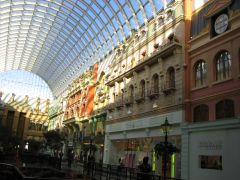
\includegraphics[width=.45\columnwidth]{Lorem}} \quad
\subfloat[Pan ma signo]
{\label{fig:example-b}%
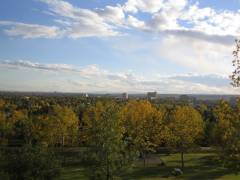
\includegraphics[width=.45\columnwidth]{Ipsum}} \\
\subfloat[Methodicamente o uno]
{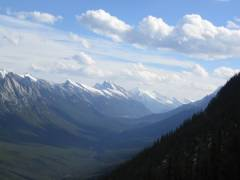
\includegraphics[width=.45\columnwidth]{Dolor}} \quad
\subfloat[Titulo debitas]
{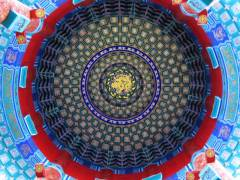
\includegraphics[width=.45\columnwidth]{Sit}}
\caption[Tu duo titulo debitas latente]{Tu duo titulo debitas latente}
\label{fig:example}
\end{figure}

Please note that the content of this section is just some dummy text. It isn't a real language.

Lorem ipsum dolor sit amet, consectetuer adipiscing elit. Ut purus elit, vestibulum ut, placerat ac, adipiscing vitae, felis. Curabitur dictum gravida mauris.

\subsection*{A subsection}

\lipsum[2]

\subsubsection*{A sub-subsection}

\lipsum[7]

\paragraph{A paragraph}
Lorem ipsum dolor sit amet, consectetuer adipiscing elit. Ut purus elit, vestibulum ut, placerat ac, adipiscing vitae, felis. Curabitur dictum gravida mauris. Nam arcu libero, nonummy eget, consectetuer id, vulputate a, magna.

\paragraph{Another paragraph}
Cras nec ante, pellentesque a nulla, cum sociis natoque penatibus et magnis dis parturient montes, nascetur ridiculus mus. Aliquam tincidunt urna

\bigskip

Donec aliquet, tortor sed accumsan bibendum, erat ligula aliquet magna, vitae ornare odio metus a mi. Morbi ac orci et nisl hendrerit mollis. Suspendisse ut massa. Cras nec ante. Pellentesque a nulla. Cum sociis natoque penatibus et magnis dis parturient montes, nascetur ridiculus mus. Aliquam tincidunt urna.

\begin{description}
\item[Mane] Lorem ipsum dolor sit amet, consectetuer adipiscing elit.
\item[Tekel] Ut purus elit, vestibulum ut, placerat ac, adipiscing vitae, felis. Curabitur dictum gravida mauris.
\item[Fares] Nam arcu libero, nonummy eget, consectetuer
id, vulputate a, magna.
\end{description}

\begin{table}
\caption{Lorem ipsum dolor sit amet}
\centering
\begin{tabular}{ll}
\toprule
\textbf{Alkaloid} & \textbf{Origin} \\
\midrule
atropine & belladonna \\
morphine & poppy \\
nicotine & tobacco \\
\bottomrule
\end{tabular}
\end{table}

Suspendisse vel felis. Ut lorem lorem, interdum eu, tincidunt sit amet, laoreet vitae, arcu. Aenean faucibus pede eu ante. Praesent enim elit, rutrum at, molestie non, nonummy vel, nisl. Ut lectus eros, malesuada sit amet, fermentum eu, sodales cursus, magna. Donec eu purus. Quisque vehicula, urna sed ultricies auctor, pede lorem egestas dui, et convallis elit erat sed nulla.

\subsection*{Some formulas}

Una formula in linea viene incorporata nel testo: $\lim_{n \to \infty}\sum_{k=1}^n \frac{1}{k^2} = \frac{\pi^2}{6}$, per esempio. Come si osserva, \LaTeX{} fa \emph{il possibile} per comprimerla e modificare il meno possibile l'interlinea nel capoverso che la contiene.
Una formula in display viene invece composta da \LaTeX{} su linee a parte, separate dal contesto con adeguati spazi bianchi per metterla in mostra e farla risaltare sulla pagina.
\begin{equation}
\lim_{n \to \infty}\sum_{k=1}^n \frac{1}{k^2}= \frac{\pi^2}{6}
\end{equation}
Come si osserva, ora la formula risulta centrata, non compressa, e tutti i suoi elementi occupano il giusto spazio con un risultato finale di grande respiro.

Integer tempus convallis augue. Etiam facilisis. Nunc elementum fermentum wisi. Aenean placerat. Ut imperdiet, enim sed gravida sollicitudin, felis odio placerat quam, ac pulvinar elit purus eget enim.

\begin{equation}
\int_a^{a+T}f(x)\,dx= \int_0^T f(x)\,dx
\qquad
\oint f(z)\,dz=2\pi i
\end{equation}

Nulla malesuada porttitor diam. Donec felis erat, congue non, volutpat at, tincidunt tristique, libero. Vivamus viverra fermentum felis. Donec non- ummy pellentesque ante.

\begin{equation}
f(x_1,\dots,x_n)=  \prod_{k=1}^n x_k
\qquad
\sum_{k=1}^n x_k^2=1
\qquad
\biggl(\sum_n x_n^2\biggr)^{1/2}
\end{equation}

\lipsum[2]

\begin{equation}
\begin{bmatrix}
a_{11} & \dots & a_{1n} \\
a_{21} & \dots & a_{2n} \\
\hdotsfor{3} \\
a_{n1} & \dots & a_{nn}
\end{bmatrix}
\end{equation}

\lipsum[4]

\begin{equation}
\lim_{x\to 0}
\frac{\sin x}{x}=1 \qquad
\lim_{n\to +\infty}f_n=\delta
\end{equation}

Fusce mauris. Vestibulum luctus nibh at lectus. Sed bibendum, nulla a faucibus semper, leo velit ultricies tellus, ac venenatis arcu wisi vel nisl. Vestibulum diam.

\begin{equation}
n!=
\begin{cases}
1       & \text{if $n=0$} \\
n(n-1)! & \text{if $n\ge 1$}
\end{cases}
\end{equation}

Ut lectus eros, malesuada sit amet, fermentum eu, sodales cursus, magna. Donec eu purus. Quisque vehicula, urna sed ultricies auctor, pede lorem egestas dui, et convallis elit erat sed nulla. Donec luctus. Curabitur et nunc. Aliquam dolor odio, commodo pretium, ultricies non, pharetra in, velit.

\begin{equation}
x_G=
\frac{\displaystyle
      \sum_{i=1}^n m_ix_i}
{\displaystyle\sum_{i=1}^n m_i}
\end{equation}

\lipsum[6]

\begin{equation}
\kappa =\frac{\xi}{E_{\textrm{max}}}
\qquad
E_{\textup{max}} =\frac{2 m_{\textup{e}} \beta^2\gamma^2 }{1 +2\gamma m_{\textup{e}}/m_{\textrm{x}} + ( m_{\textup{e}}/m_{\textup{x}})^2}
\end{equation}

\lipsum[8]

% !TEX TS-program = pdflatex
% !TEX root = ../tesi.tex

%************************************************
\chapter{Code}
\label{chp:code}
%************************************************

\lstset{numbers=left,
    numberstyle=\scriptsize,
    stepnumber=1,
    numbersep=8pt
}



Package announcement and request for necessary packages.
\begin{lstlisting}[firstnumber=1]
\NeedsTeXFormat{LaTeX2e}
\ProvidesPackage{arsclassica}[2017/02/01]
\RequirePackage{classicthesis}
\RequirePackage{caption}
\end{lstlisting}



Text body size.
\begin{lstlisting}
\areaset[current]{370pt}{784pt}
\end{lstlisting}



Use of Iwona as font sans serif.
\begin{lstlisting}
\renewcommand{\sfdefault}{iwona}
\end{lstlisting}



Customized chapter numbers.
\begin{lstlisting}
\let\chapterNumber\undefined
\ifct@eulerchapternumbers
\newfont{\chapterNumber}{eurb10 scaled 5000}%
\else
\newfont{\chapterNumber}{pplr9d scaled 5000}%
\fi
\end{lstlisting}



Smallcaps sans serif.
\begin{lstlisting}
\ifthenelse{\boolean{@minionprospacing}}%
{%
  \DeclareRobustCommand{\spacedallcaps}[1]{\sffamily%
  \textssc{\MakeTextUppercase{#1}}}%
  \DeclareRobustCommand{\spacedlowsmallcaps}[1]%
  {\sffamily\textssc{\MakeTextLowercase{#1}}}%
}{%
  \ifthenelse{\boolean{@pdfspacing}}%
  {%
    \microtypesetup{expansion=false}%
    \DeclareRobustCommand{\spacedallcaps}[1]%
    {\sffamily\textls[160]{\MakeTextUppercase{#1}}}%
    \DeclareRobustCommand{\spacedlowsmallcaps}[1]%
    {\sffamily\textls[80]{\scshape\MakeTextLowercase{#1}}}%
  }{%
    \RequirePackage{soul}
    \sodef\allcapsspacing{\sffamily\upshape}%
    {0.15em}{0.65em}{0.6em}%
    \sodef\lowsmallcapsspacing{\sffamily\scshape}%
    {0.075em}{0.5em}{0.6em}%
    \DeclareRobustCommand{\spacedallcaps}[1]%
    {\MakeTextUppercase{\allcapsspacing{#1}}}%
	\DeclareRobustCommand{\spacedlowsmallcaps}[1]%
	{\MakeTextLowercase{\textsc%
	   {\lowsmallcapsspacing{#1}}}}%
  }%
}
\end{lstlisting}



Semi-transparent headlines and page numbers in Iwona.
\begin{lstlisting}
\renewcommand{\sectionmark}[1]{\markright{\textsc%
{\MakeTextLowercase{\thesection}} \spacedlowsmallcaps{#1}}}
\lehead{\mbox{\llap{\small\thepage\kern1em\color{halfgray}\vline}%
\color{halfgray}\hspace{0.5em}\headmark\hfil}}
\rohead{\mbox{\hfil{\color{halfgray}%
\headmark\hspace{0.5em}}%
\rlap{\small{\color{halfgray}\vline}\kern1em\thepage}}}
\renewcommand{\headfont}{\normalfont\sffamily}
\renewcommand{\pnumfont}{\small\sffamily}
\end{lstlisting}



Sectioning unit titles and description list labels in Iwona.
\begin{lstlisting}
\RequirePackage{titlesec}
    % parts
    \ifthenelse{\boolean{@parts}}%
    {%
    \titleformat{\part}[display]
        {\normalfont\centering\large}%
        {\thispagestyle{empty}\partname~\thepart}{1em}%
        {\color{Maroon}\spacedallcaps}
    }{\relax}
    % chapters
    \ifthenelse{\boolean{@linedheaders}}%
    {%
    \titleformat{\chapter}[display]%
       {\relax}{\raggedleft{\color{halfgray}%
       \chapterNumber\thechapter} \\ }{0pt}%
       {\titlerule\vspace*{.9\baselineskip}\raggedright%
       \spacedallcaps}%
       [\normalsize\vspace*{.8\baselineskip}\titlerule]%
    }{%
    \titleformat{\chapter}[block]%
       {\normalfont\Large\sffamily}%
       {{\color{halfgray}\chapterNumber\thechapter%
       \hspace{10pt}\vline}  }{10pt}%
       {\spacedallcaps}}
    % sections
    \titleformat{\section}
       {\normalfont\Large\sffamily}{\textsc%
       {\MakeTextLowercase{\thesection}}}%
       {1em}{\spacedlowsmallcaps}
    % subsections
       \titleformat{\subsection}
       {\normalfont\sffamily\bfseries}{\textsc{\MakeTextLowercase%
       {\thesubsection}}}{1em}{\normalsize}
    % subsubsections
    \titleformat{\subsubsection}
       {\normalfont\sffamily\bfseries\itshape}{\textsc%
       {\MakeTextLowercase{\thesubsubsection}}}%
       {1em}{\normalsize\itshape}
    % paragraphs
    \titleformat{\paragraph}[runin]
       {\normalfont\normalsize\sffamily\bfseries}{\textsc%
       {\MakeTextLowercase{\theparagraph}}}%
       {0pt}{\spacedlowsmallcaps}
    % description labels
    \renewcommand{\descriptionlabel}[1]{\hspace*{\labelsep}%
    \bfseries\spacedlowsmallcaps{#1}}
    \titlespacing*{\chapter}{0pt}{1\baselineskip}{2\baselineskip}
    \titlespacing*{\section}{0pt}{2\baselineskip}%
       {.8\baselineskip}[\marginparsep]
    \titlespacing*{\subsection}{0pt}{1.5\baselineskip}%
       {.8\baselineskip}[\marginparsep]
    \titlespacing*{\paragraph}{0pt}{1\baselineskip}{1\baselineskip}

    \newcommand\formatchapter[1]{%
    \vbox to \ht\strutbox{
    \setbox0=\hbox{\chapterNumber\thechapter\hspace{10pt}\vline\ }
    \advance\hsize-\wd0 \advance\hsize-10pt\raggedright
    \spacedallcaps{#1}\vss}}
    \titleformat{\chapter}[block]
       {\normalfont\Large\sffamily}
       {\textcolor{halfgray}{\chapterNumber\thechapter}
       \hspace{10pt}\vline\ }{10pt}
    {\formatchapter}

    \clearscrplain
    \rofoot[\mbox{\makebox[0pt][l]{\kern1em\thepage}}]{}
\end{lstlisting}



Itemize lists with semi-transparent labels.
\begin{lstlisting}
\renewcommand\labelitemi{\color{halfgray}$\bullet$}
\end{lstlisting}



Caption settings.
\begin{lstlisting}
\captionsetup{format=hang,font=small,labelfont={sf,bf}}
\captionsetup[table]{skip=\medskipamount}
\end{lstlisting}



Hyper-reference settings.
\begin{lstlisting}
\hypersetup{
    colorlinks=true, linktocpage=true, pdfstartpage=1,
    pdfstartview=FitV, breaklinks=true, pdfpagemode=UseNone,
    pageanchor=true, pdfpagemode=UseOutlines,
    plainpages=false, bookmarksnumbered,
    bookmarksopen=true, bookmarksopenlevel=1,
    hypertexnames=true, pdfhighlight=/O,
    urlcolor=webbrown, linkcolor=RoyalBlue,
    citecolor=webgreen,
    hyperfootnotes=false, pdfpagelabels,
    pdfcreator={pdfLaTeX},
    pdfproducer={LaTeX with ArsClassica}
}
\end{lstlisting}

\clearpage
% !TEX TS-program = pdflatex
% !TEX root = ../tesi.tex

%*******************************************************
% Bibliography
%*******************************************************
\nocite{*}
\printbibliography

\end{document}
